\documentclass[runningheads]{comsis2}

%% Necessary definitions for the running heads
\def\journalissue{Computer Science and Information Systems 00(0):0000--0000}
\def\paperidnum{https://doi.org/10.2298/CSIS123456789X}
\setcounter{page}{1}

%% Use this to show line numbers (and remove only in the final camera-ready version)
\usepackage[pagewise]{lineno}
\linenumbers
\usepackage{hyperref}
\usepackage{verbatim}
\usepackage{graphicx}


%%%%% NEW PACKAGES 
\usepackage{graphicx}
\usepackage{color, colortbl}
\graphicspath{ {./figures/} }

\definecolor{lightgreen}{rgb}{0.82, 0.94, 0.75}
\definecolor{lightorange}{rgb}{0.98, 0.84, 0.65}
\newcommand*{\Comb}[2]{{}C^{#1}_{#2}}%
%%%%%%%

\title{Logical dependencies: extraction from the versioning system and an example of usage
\footnote{If this is an extended version of a conference paper, it should be clearly stated here.}}

%% Use this if the title is too long for the running heads
\titlerunning{Logical dependencies in practice}

\author{Adelina Stana\inst{1} \and Ioana Sora\inst{2}}

%% Use this the list of authors is too long for the running heads
%\authorrunning{First Author et al.}

\institute{Stana Adelina Diana\\
  Address\\
  \email{stana.adelina.diana@gmail.com}
  \and
  Sora Ioana\\
  Address\\
  \email{ioana.sora@cs.upt.ro}}

\begin{document}

\maketitle

\begin{abstract}
One of the biggest problems when it comes to legacy software systems is the lack of modernization. A legacy software system is an obsolete system that might still be in use and satisfy the organization's needs but due to the lack of modernization, it has a high maintenance cost. One solution is to modernize or refactor the system and to do that the developers must have a good understanding of the system. Here comes one other problem of the legacy software systems, the lack of up-to-date documentation or the lack of documentation. The solution for this problem is to analyze the legacy software system in order to gain more knowledge about the system and how the system works. Our approach is to analyze the legacy software system by using historical information extracted from the versioning systems.

\vspace{6pt}\textbf{Keywords:} logical dependencies, versioning system, key classes.
\end{abstract}


\section{The concept of logical dependencies}

A logical dependency between two software entities (classes, modules, interfaces, etc. ) signals that those entities in some way depend on one another. 

The concept of logical coupling (dependency) was first introduced by Gall \cite{Gall:1998:DLC:850947.853338}. They defined the logical coupling between two modules as the fact that the modules repeatedly change together during the historical evolution of the software system.

To define the logical dependencies, we have first to define the co-changing pairs. A \textit{co-changing pair} are two software entities that update together in the same commit. For example, a commit that contains seven entities will generate 21 co-changing pairs ($\Comb{n}{k}=\frac{n!}{k!(n-k)!} = \frac{7!}{2!(5)!} = 21$).


After extraction, some co-changing pairs are removed by passing them through various filters (filtering phase). The \textit{logical dependencies} are those co-changing pairs that remain after the filtering phase. Another reason for the filtering is to decrease the size of processed data; a commit with 1030 entities will produce over half a million co-changing pairs. These kinds of commits are, in most cases, not code-related, so the co-changing pairs extracted from this kind of commit have nothing to do with the code.

Previously, we tried to obtain reliable logical dependencies from co-changing pairs by applying different types of filters like the occurrence filter and commit size filter \cite{saci19}, \cite{enase19}. The main disadvantage of the occurrence filter was that it did not work well for systems with few commits.

Currently, we aim to refine the filtering method with a new filter that can be applied for all sorts of commit history sizes. This new filter will be used together with a filter previously explored, the commit size filter \cite{enase19}.

\subsection{Commit size filter}

The commit size filter filters out all co-changing pairs from commits with more than 10 files changed. We consider that commits with more than 10 files changed tend to be code unrelated; we studied the commit size trend from serval git open-source repositories, and we concluded that most of the commits contain less than ten files. On average, only 10 \% of the total commits have more than ten files changed. 

This filter will also prevent the volume of data processed from going out of proportion. In some of the repositories studied, we found commits with more than 1000 files; these commits could generate over half a million co-changing pairs if the commit size filter is not applied. 

\subsection{Connection strength filter}

This filter is new for our research regarding logical dependencies and is based on the experience with other filters applied unsuccessfully. 

One important conclusion drawn from other types of filtering that we tried over time is that setting a hard threshold for a filter is not always a good idea. A certain threshold can work well with a medium/large-sized system but, when applied to a small-sized system, can reduce the co-changes filtered to 0. This made us realize that we need a filter that is computed according to the system's specifications. 

We will call this filter, the connection strength filter and, it is applied after the commit size filter. To determine the connection strength, we first need to calculate the connection factors of both entities that form a co-changing pair.

Assuming that we have a co-changing pair formed by entities A and B, the connection factor of entity A with entity B is the percentage from the total commits involving A that contains entity B. The connection factor of entity B with entity A is the percentage from the total commits involving B also containing entity A.

\begin{equation}
 connection\ factor\ for\ A = \frac{100 * commits\ involving\ A\ and\ B}{total\ nr\ of\ commits\ involving\ A}
\end{equation}

\begin{equation}
 connection\ factor\ for\ B = \frac{100 * commits\ involving\ A\ and\ B}{total\ nr\ of\ commits\ involving\ B}
\end{equation}

We calculated the connection factor for each entity involved in a co-changing pair and filtered the co-changing pairs based on it. The rule set is that both entities that form a co-changing pair had to have a connection factor with each other greater than a threshold value.

As a practical example, if the pair formed by A and B update together 7 times and the total number of commits involving A is 20 and involving B is 7, then the factor for A is 35 and for B is 100. If the connection strength threshold is set to 50, that means that this co-changing pair will be filtered out because the factor of A is smaller than the threshold. 

Since the factors can vary from 0 to 100, for this filter, we started with a threshold value of 10 and incremented it by 10 until we reached 100. And we want to see how the threshold value affects the number of co-changing pairs left. 

In figure \ref{fig:strength_overview} we plot the number of structural dependencies, co-changing pairs before filtering, and co-changing pairs after filtering with different threshold values for two systems, one small-sized and one medium-sized. As can be observed, with this filter, the small-sized system didn't lose all the co-changing pairs once with the filtering. 

We compare the number of remaining co-changing pairs with the number of structural dependencies because according to surveys \cite{Shtern:2012:CMS:2332427.2332428}, \cite{sar}, the main reason why logical dependencies (a.k.a filtered co-changes) are not used together with structural dependencies is because of their size. So, it is essential to get an overview of the comparison between the co-changing pairs number and the structural dependencies number at each filtering step.

\begin{figure}
\centering
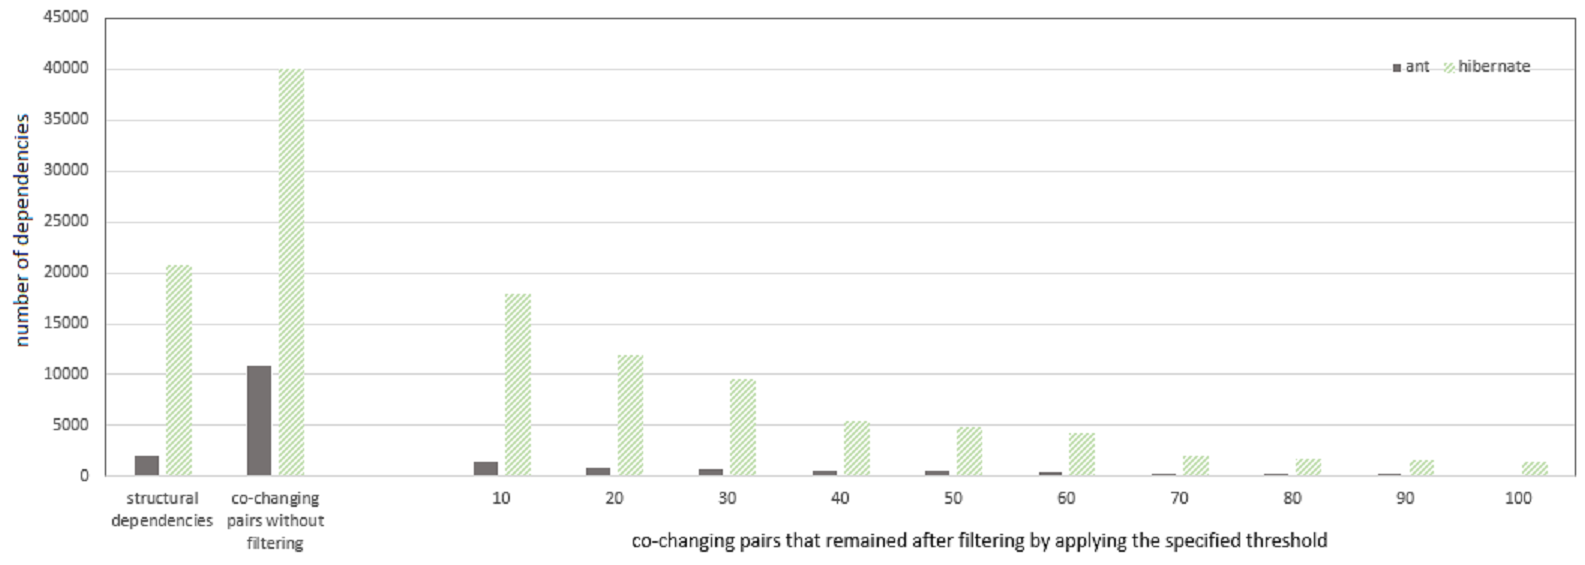
\includegraphics[width=\textwidth]{strength_overview.PNG}
\caption{Overview of the impact of connection strength filtering on the number of co-changing pairs. }
\label{fig:strength_overview}
\centering
\end{figure}


\begin{figure}
\centering
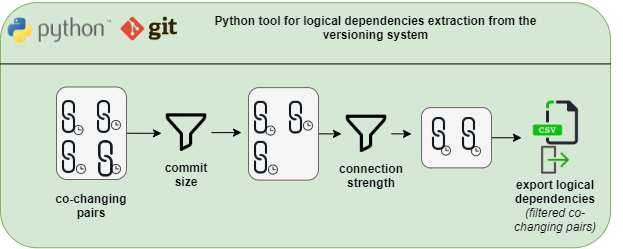
\includegraphics[width=\textwidth]{ld_workflow.png}
\caption{Workflow for logical dependencies extraction.}
\label{fig:workflow_key}
\centering
\end{figure}

The co-changing pairs that remain after filtering, can be called logical dependencies. The entire process of extracting co-changing pairs from the versioning system, filter them, and export the remaining ones is done with a tool written in Python. The tool's workflow is presented in figure \ref{fig:workflow_key}.

After this step, we will continue our research by using the logical dependencies obtained with different threshold values and see which threshold value performs the best. Up until now, we only looked at the size of the logical dependencies and decided if a filter is good or not. But now, we can also look at the results obtained by using the logical dependencies and decide.





\section{Key classes: baseline versus current approach}
\label{sec:baseline_approach}

Zaidman et al \cite{ZaidmanJurnal} were the first to introduce the concept of key classes and it refers to classes that can be found in documents written to provide an architectural overview of the system or an introduction to the system structure. 
Tahvildari and Kontogiannis have a more detailed definition regarding key classes concept: “Usually, the most important concepts of a system are implemented by very few key classes which can be characterized by the specific properties. These classes, which we refer to as key classes, manage many other classes or use them in order to implement their functionality. The key classes are tightly coupled with other parts of the system. Additionally, they tend to be rather complex, since they implement much of the legacy system’s functionality” \cite{Tahvildari2004ImprovingDQ}.


The key class identification can be done by using different algorithms with different inputs. In the research of Osman et al., the key class identification is made by using a machine learning algorithm and class diagrams as input for the algorithm \cite{6676885}. Thung et al. builds on top of Osman et al.’s approach and adds network metrics and optimistic classification in order to detect key classes \cite{rocclasification}.  

Zaidman et al. use a webmining algorithm and dynamic analysis of the source code to identify the key classes \cite{ZaidmanJurnal}.

\subsection{Baseline approach}
We use the research of I. Sora et al \cite{Finding-key-classes} as a baseline for our research involving the usage of logical dependencies to find key classes. 

Sora et al. used the static analysis of the source code, a page ranking algorithm and other class attributes to find key classes \cite{PagerankENASE}, \cite{enase15}, \cite{SoraSpringer}, \cite{PagerankSACI},\cite{Finding-key-classes}.
The page ranking algorithm is a customization of PageRank, the algorithm used to rank web pages \cite{ilprints422} and works based on a recommendation system. If one node has a connection with another node, then it recommends the second node. In previous works, connections are established based on structural dependencies extracted from static code analysis. If A has a structural dependency with B, then A recommends B, and also B recommends A.

The ranking algorithm ranks all the classes from the source code of the system analyzed according to their importance. To identify the important classes from the rest of the classes a threshold for TOP classes from the top of the ranking is set. The TOP threshold value can go from 1 to the total number of classes found in the system. 



\subsection{Current approach}

The baseline approach uses a tool that takes as an input the source code of the system and applies ranking strategies to rank the classes according to their importance. 

In order to rank the classes according to their importance, different class metrics are used \cite{Ding2016AnIA}, \cite{ZaidmanJurnal}, \cite{PAN2018188}. Below are some of the class metrics used in the baseline approach and our current research to rank the classes according to their importance. We use only a subset of the metrics used in previous research because the extracted logical dependencies are undirected.


The class metrics used can be separated into two categories: class connection metrics and class PageRank values.
The class connection metrics are CONN-TOTAL-W, which is the total weight of all connections of the class, and CONN-TOTAL, the total number of distinct classes that a class uses or are used by a class \cite{Finding-key-classes}.

Previous research used PageRank values computed on both directed and undirected, weighted and unweighted graphs. In the current research, we used the PR, which is the PageRank value computed on the directed and unweighted graph. The PR-U, which is the value computed on the undirected and unweighted graph, and PR-U2-W, the value computed on the weighted graph with back-recommendations \cite{PagerankENASE}, \cite{enase15}, \cite{Finding-key-classes}, \cite{PagerankSACI}.


Based on the class attributes presented, all the classes of the system are ranked. 

We modified the tool used by the baseline approach to take also the logical dependencies as input; the rest of the workflow remained the same as the baseline approach. The entire workflow is presented in figure \ref{fig:baseline_approach}.

\begin{figure}
\centering
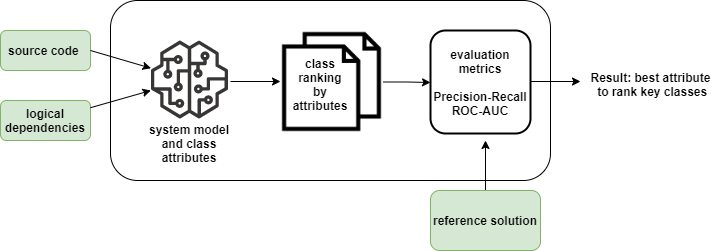
\includegraphics[width=\textwidth]{current_approach.PNG}
\caption{Overview of the current approach.}
\label{fig:baseline_approach}
\centering
\end{figure}
%%%

\section{Metrics for results evaluation}
\label{sec:evalmetrics}
To evaluate the quality of the key classes ranking algorithm and solution produced, the key classes found by the algorithm are compared with a reference solution. The reference solution is extracted from the developer documentation.  Classes mentioned in the documentation are considered key classes and form the reference solution (ground truth) used for validation \cite{7551990}. 

For the comparison between both solutions, a classification model is used. The quality of the solution produced is evaluated by using the Receiver Operating Characteristic Area Under Curve (ROC-AUC) metric, a metric that evaluates the performance of a classification model.


\textit{Receiver Operating Characteristic Area Under Curve}


The ROC graph is a two-dimensional graph that has on the X-axis plotted the false positive rate and on the Y-axis the true positive rate. By plotting the true positive rate and the false positive rate at thresholds that vary between a minimum and a maximum possible value we obtain the ROC curve. The area under the ROC curve is called Area Under the Curve (AUC).

The true positive rate of a classifier is calculated as the division between the number of true positive results identified and all the positive results identified:

\begin{equation}
 True\ positive\ rate (TPR) = \frac{TP}{TP+FN}
\end{equation}
The false positive rate of a classifier is calculated as the division between the number of false positive results identified and all the negative results identified:

\begin{equation}
 False\ positive\ rate (FPR) = \frac{FP}{FP+TN}
\end{equation}

The baseline approach not only identifies the key classes but also evaluates the performance of the solution produced. To differentiate the important (key) classes from the rest of the classes, a TOP threshold for the top classes found is set. The threshold vary between 20 and 30 classes.

The true positives (TP) are the classes found in the reference solution and also in the top TOP ranked classes. False positives (FP) are the classes that are not in the reference solution but are in the TOP ranked classes.
True Negatives (TN) are classes that are found neither in the reference solution nor in the TOP ranked classes. False Negatives (FN) are classes that are found in the reference solution but not found in the TOP ranked classes.



In multiple related works, the ROC-AUC metric has been used to evaluate the results for finding key classes of software systems.
For a classifier to be considered good, its ROC-AUC metric value should be as close to 1 as possible, when the value is 1 then the classifier is considered to be perfect.

Osman et al. obtained in their research an average Area Under the Receiver Operating Characteristic Curve (ROC-AUC) score of 0.750 \cite{6676885}. Thung et al. obtained an average ROC-AUC score of 0.825 \cite{rocclasification}  and Sora et al. (the baseline) obtained an average ROC-AUC score of 0.894 \cite{Finding-key-classes}.


\section{Data set used}
\label{sec:dataset}
In this section, we will look over all the systems studied in the baseline research presented in section \ref{sec:baseline_approach}, and we will try to identify the systems that could be used also in our current research involving logical dependencies.


The research of I. Sora et al \cite{Finding-key-classes} takes into consideration structural public dependencies that are extracted using static analysis techniques and was performed on the object-oriented systems presented in table \ref{tab:gitfoundsystems}.

The requirements for a system to qualify as suited for investigations using logical dependencies are: has to be on GitHub, has to have releases to identify a specific version (previous research was done only on specific releases), and also, has to have a significant number of commits. 
From the total of 14 object-oriented systems listed in the paper \cite{Finding-key-classes}, 13 of them have repositories in Github \ref{tab:gitfoundsystems}. And from the found repositories, only 6 repositories have the same release tag as the specified version in previous research.
The commits number found on the remaining 6 repositories varies from 19108 commits for Tomcat Catalina to 149 commits for JHotDraw. In order to have more accurate results, we need a significant number of commits, so we reached the conclusion that only 3 systems can be used for key classes detection using logical dependencies: Apache Ant, Hibernate, and Tomcat Catalina.  From all the systems mentioned in table \ref{tab:gitfoundsystems} Apache Ant is the most used and analyzed in other  works \cite{enase19}, \cite{7332515}, \cite{1402122}, \cite{Kamran2016IdentificationOC}.

\begin{table}
\renewcommand{\arraystretch}{1}
\caption{Found systems and versions of the systems in GitHub. }
\label{tab:gitfoundsystems}
\centering
\begin{tabular}{lllll}
\hline
ID	&	System	&	Version	&	Release Tag name	&	Commits number	\\
\hline
Sl	&	Apache Ant	&	1.6.1	&	rel/1.6.1	&	6713	\\
S2	&	Argo UML	&	0.9.5	&	not found	&	0	\\
S3	&	GWT Portlets	&	0.9.5 beta	&	not found	&	0	\\
S4	&	Hibernate 	&	5.2.12	&	5.2.12	&	6733	\\
S5	&	javaclient	&	2.0.0	&	not found	&	0	\\
S6	&	jEdit	&	5.1.0	&	not found	&	0	\\
S7	&	JGAP	&	3.6.3	&	not found	&	0	\\
S8	&	JHotDraw	&	6.0b.1	&	not found	&	149	\\
S9	&	JMeter	&	2.0.1	&	v2\_1\_1	&	2506	\\
S10	&	Log4j	&	2.10.0	&	v1\_2\_10-recalled	&	634	\\
S11	&	Mars	&	3.06.0	&	not found	&	0	\\
S12	&	Maze	&	1.0.0	&	not found	&	0	\\
S13	&	Neuroph	&	2.2.0	&	not found	&	0	\\
S14	&	Tomcat Catalina	&	9.0.4	&	9.0.4	&	19108	\\
S15	&	Wro4J	&	1.6.3	&	v1.6.3	&	2871	\\
\hline
\end{tabular}
\end{table}




\section{Measurements using logical dependencies}
\label{sec:current_measurements}

As we mentioned in the beginning the purpose is to check if the logical dependencies can improve key class detection. 

As presented in section \ref{sec:baseline_approach}, the key class detection was done by using structural dependencies of the system. 
In this section, we will use the same tool used in the baseline approach presented in section \ref{sec:baseline_approach}, and we will add a new input to it, the logical dependencies. 

Below is a comparison between the new approach and baseline approach, how we collect the logical dependencies, the results obtained previously, and the new results obtained. 
The new results are separated into two categories, the results obtained by using structural and logical dependencies and the results obtained by using only logical dependencies. 


\subsection{Measurements using only the baseline approach}


In table \ref{tab:previousresults} are presented the ROC-AUC values for different attributes computed for the systems Ant, Tomcat Catalina, and Hibernate by using the baseline approach. We intend to compare these values with the new values obtained by using also logical dependencies in key class detection.

\begin{table}[!h]
\renewcommand{\arraystretch}{1}
\caption{ROC-AUC metric values extracted. }
\label{tab:previousresults}
\centering
\scalebox{0.9}{
\begin{tabular}{|c|ccc|}
\hline
Metrics &	Ant	&	Tomcat Catalina	&	Hibernate	\\
\hline

PR\_U2\_W	&	0.95823	&	0.92341	&	0.95823	\\
PR	&	0.94944	&	0.92670	&	0.94944	\\
PR\_U	&	0.95060	&	0.93220	&	0.95060	\\
CONN\_TOTAL\_W	&	0.94437	&	0.92595	&	0.94437	\\
CONN\_TOTAL	&	0.94630	&	0.93903	&	0.94630	\\

\hline
\end{tabular}
}
\end{table}





\subsection{Measurements using combined structural and logical dependencies}

The tool used in the baseline approach runs a graph-ranking algorithm. 
The graph used contains the structural dependencies extracted from static source code analysis.
Each edge in the graph represents a dependency, the entities that form a structural dependency are represented as vertices in the graph. 
As mentioned in section \ref{sec:baseline_approach}, we modified the tool to read also logical dependencies and add them to the graph. 
In this section, we add in the graph the logical dependencies together with the structural dependencies. 

In tables \ref{tab:measurementscombined:ant}, \ref{tab:measurementscombined:tomcat}, and \ref{tab:measurementscombined:hibernate}, on each line, we have the metric that is calculated and on each column, we have the connection strength threshold that was applied to the logical dependencies used in identifying the key classes.
We started with logical dependencies that have a connection strength greater than 10\%, which means that in at least 10\% of the commits involving A or B, A and B update together. Then we increased the threshold value by 10 until we remained only with entities that update in all the commits together. The last column contains the results obtained previously by the tool by only using structural dependencies.

As for the new results obtained by combining structural and logical dependencies, highlighted with orange are the values that are close to the previously registered values but did not surpass them. Highlighted with green are values that are better than the previously registered values. At this step, we can also observe that for all three systems measured in tables \ref{tab:measurementscombined:ant}, \ref{tab:measurementscombined:tomcat}, and \ref{tab:measurementscombined:hibernate}, the best values obtained are for connection strength between 40-70\%.

\begin{table}[!h]
\renewcommand{\arraystretch}{1}
\caption{Measurements for Ant using structural and logical dependencies combined}
\label{tab:measurementscombined:ant}
\centering
\begin{tabular}{|c|cccccccccc|c|}
\hline
Metrics &	$\geq10\%$	&	$\geq20\%$		&	$\geq30\%$		&	$\geq40\%$		&	$\geq50\%$		&	$\geq60\%$		&	$\geq70\%$		&	$\geq80\%$		&	$\geq90\%$		&	$\geq100\%$		&	Baseline \\
\hline

PR\_U2\_W	&	0.924	&	0.925	&	0.926	&	0.927	&	0.927	&	0.927	&	\cellcolor{lightgreen}0.929	&	0.928	&	0.928	&	0.928	&	0.929	\\
PR	&	0.914	&	0.854	&	0.851	&	\cellcolor{lightgreen}0.866	&	\cellcolor{lightgreen}0.876	&	\cellcolor{lightgreen}0.882	&	\cellcolor{lightgreen}0.887	&	0.854	&	0.852	&	0.852	&	0.855	\\
PR\_U	&	0.910	&	0.930	&	0.933	&	0.933	&	\cellcolor{lightgreen}0.935	&	\cellcolor{lightgreen}0.934	&	\cellcolor{lightgreen}0.939	&	0.933	&	0.933	&	0.933	&	0.933	\\
CON\_T\_W	&	0.924	&	0.928	&	0.931	&	0.932	&	0.933	&	0.934	&	\cellcolor{lightgreen}0.936	&	0.934	&	0.934	&	0.934	&	0.934	\\
CON\_T	&	0.840	&	0.886	&	0.904	&	0.909	&	0.915	&	0.923	&	0.932	&	0.935	&	\cellcolor{lightorange}0.936	&	\cellcolor{lightorange}0.936	&	0.942	\\

\hline
\end{tabular}
\end{table}


\begin{table}[!h]
\renewcommand{\arraystretch}{1}
\caption{Measurements for Tomcat using structural and logical dependencies combined}
\label{tab:measurementscombined:tomcat}
\centering
\begin{tabular}{|c|cccccccccc|c|}
\hline
Metrics &	$\geq10\%$	&	$\geq20\%$		&	$\geq30\%$		&	$\geq40\%$		&	$\geq50\%$		&	$\geq60\%$		&	$\geq70\%$		&	$\geq80\%$		&	$\geq90\%$		&	$\geq100\%$		&	Baseline \\
\hline

PR\_U2\_W	&	0.910	&	0.917	&	0.923	&	\cellcolor{lightgreen}0.924	&	\cellcolor{lightgreen}0.924	&	\cellcolor{lightgreen}0.924	&	\cellcolor{lightgreen}0.924	&	\cellcolor{lightgreen}0.924	&	\cellcolor{lightgreen}0.924	&	\cellcolor{lightgreen}0.924	&	0.923	\\
PR	&	0.811	&	0.800	&	0.815	&	0.834	&	0.847	&	0.852	&	0.853	&	0.858	&	0.858	&	0.858	&	0.927	\\
PR\_U	&	0.910	&	0.921	&	0.931	&	\cellcolor{lightgreen}0.933	&	\cellcolor{lightgreen}0.933	&	0.932	&	\cellcolor{lightgreen}0.933	&	0.932	&	0.932	&	0.932	&	0.932	\\
CON\_T\_W	&	0.914	&	0.920	&	0.924	&	\cellcolor{lightorange}0.926	&	0.926	&	0.926	&	0.926	&	0.926	&	0.926	&	0.926	&	0.926	\\
CON\_T	&	0.868	&	0.906	&	0.930	&	0.936	&	0.937	&	\cellcolor{lightorange}0.938	&	0.938	&	0.938	&	0.938	&	0.938	&	0.939	\\
																												

\hline
\end{tabular}
\end{table}


\begin{table}[!h]
\renewcommand{\arraystretch}{1}
\caption{Measurements for Hibernate using structural and logical dependencies combined}
\label{tab:measurementscombined:hibernate}
\centering
\begin{tabular}{|c|cccccccccc|c|}
\hline
Metrics &	$\geq10\%$	&	$\geq20\%$		&	$\geq30\%$		&	$\geq40\%$		&	$\geq50\%$		&	$\geq60\%$		&	$\geq70\%$		&	$\geq80\%$		&	$\geq90\%$		&	$\geq100\%$		&	Baseline \\
\hline

PR\_U2\_W	&	0.954	&	0.957	&	\cellcolor{lightorange}0.958	&	0.958	&	0.958	&	0.958	&	0.958	&	0.958	&	0.958	&	0.958	&	0.958	\\
PR	&	0.929	&	0.929	&	0.933	&	0.939	&	0.939	&	0.946	&	\cellcolor{lightorange}0.947	&	0.947	&	0.947	&	0.947	&	0.949	\\
PR\_U	&	0.942	&	0.947	&	0.948	&	0.949	&	0.949	&	\cellcolor{lightorange}0.950	&	0.950	&	0.950	&	0.950	&	0.950	&	0.951	\\
CON\_T\_W	&	0.939	&	0.942	&	0.943	&	0.944	&	0.944	&	\cellcolor{lightgreen}0.945	&	\cellcolor{lightgreen}0.945	&	\cellcolor{lightgreen}0.945	&	\cellcolor{lightgreen}0.945	&	\cellcolor{lightgreen}0.945	&	0.944	\\
CON\_T	&	0.924	&	0.933	&	0.938	&	0.941	&	0.941	&	0.944	&	\cellcolor{lightorange}0.945	&	0.945	&	0.945	&	0.945	&	0.946	\\


\hline
\end{tabular}
\end{table}

\subsection{Measurements using only logical dependencies}
In the previous section, we added in the graph based on which the ranking algorithm works the logical and structural dependencies. In the current section, we will add only the logical dependencies to the graph.

In tables \ref{tab:measurementshistory:ant}, \ref{tab:measurementshistory:tomcat}, and \ref{tab:measurementshistory:hibernate}, are presented the results obtained by using only logical dependencies to detect key classes. The measurements obtained are not as good as using logical and structural dependencies combined or using only structural dependencies. But, all the values obtained are above 0.5, which means that a good part of the key classes is detected by only using logical dependencies.  As mentioned in section \ref{sec:evalmetrics}, a classifier is good if it has the ROC-AUC value as close to 1 as possible. 


One possible explanation for the less performing results is that the key classes may have a better design than the rest of the classes, which means that are less prone to change. If the key classes are less prone to change, this implies that the number of dependencies extracted from the versioning system can be less than for other classes.

\begin{table}[!h]
\renewcommand{\arraystretch}{1}
\caption{Measurements for Ant using only logical dependencies}
\label{tab:measurementshistory:ant}
\centering
\begin{tabular}{|c|cccccccccc|c|}
\hline
Metrics &	$\geq10\%$	&	$\geq20\%$		&	$\geq30\%$		&	$\geq40\%$		&	$\geq50\%$		&	$\geq60\%$		&	$\geq70\%$		&	$\geq80\%$		&	$\geq90\%$		&	$\geq100\%$		&	Baseline \\
\hline

PR\_U2\_W	&	0.720	&	0.627	&	0.718	&	0.703	&	0.732	&	0.824	&	0.852	&	\cellcolor{lightorange}0.881	&	0.876	&	0.876	&	0.929	\\
PR	&	0.720	&	0.627	&	0.718	&	0.703	&	0.732	&	0.824	&	0.852	&	\cellcolor{lightorange}0.881	&	0.876	&	0.876	&	0.855	\\
PR\_U	&	0.720	&	0.627	&	0.718	&	0.703	&	0.732	&	0.824	&	0.852	&	\cellcolor{lightorange}0.881	&	0.876	&	0.876	&	0.933	\\
CON\_T\_W	&	0.722	&	0.581	&	0.644	&	0.676	&	0.727	&	0.819	&	0.842	&	0.874	&	\cellcolor{lightorange}0.876	&	0.876	&	0.934	\\
CON\_T	&	0.722	&	0.581	&	0.644	&	0.676	&	0.727	&	0.819	&	0.842	&	0.874	&	\cellcolor{lightorange}0.876	&	0.876	&	0.942	\\

\hline
\end{tabular}
\end{table}


\begin{table}[!h]
\renewcommand{\arraystretch}{1}
\caption{Measurements for Tomcat using only logical dependencies}
\label{tab:measurementshistory:tomcat}
\centering
\begin{tabular}{|c|cccccccccc|c|}
\hline
Metrics &	$\geq10\%$	&	$\geq20\%$		&	$\geq30\%$		&	$\geq40\%$		&	$\geq50\%$		&	$\geq60\%$		&	$\geq70\%$		&	$\geq80\%$		&	$\geq90\%$		&	$\geq100\%$		&	Previous \\
\hline

PR\_U2\_W	&	0.672	&	0.656	&	0.645	&	0.697	&	0.754	&	0.776	&	0.786	&	\cellcolor{lightorange}0.799	&	0.799	&	0.799	&	0.923	\\
PR	&	0.685	&	0.643	&	0.642	&	0.697	&	0.754	&	0.776	&	0.786	&	\cellcolor{lightorange}0.799	&	0.799	&	0.799	&	0.927	\\
PR\_U	&	0.685	&	0.643	&	0.644	&	0.697	&	0.754	&	0.776	&	0.786	&	\cellcolor{lightorange}0.799	&	0.799	&	0.799	&	0.932	\\
CON\_T\_W	&	0.694	&	0.636	&	0.636	&	0.697	&	0.754	&	0.776	&	0.786	&	\cellcolor{lightorange}0.799	&	0.799	&	0.799	&	0.926	\\
CON\_T	&	0.654	&	0.611	&	0.636	&	0.697	&	0.754	&	0.776	&	0.786	&	\cellcolor{lightorange}0.799	&	0.799	&	0.799	&	0.939	\\

				
\hline
\end{tabular}

\end{table}


\begin{table}[!h]
\renewcommand{\arraystretch}{1}
\caption{Measurements for Hibernate using only logical dependencies}
\label{tab:measurementshistory:hibernate}
\centering
\begin{tabular}{|c|cccccccccc|c|}
\hline
Metrics &	$\geq10\%$	&	$\geq20\%$		&	$\geq30\%$		&	$\geq40\%$		&	$\geq50\%$		&	$\geq60\%$		&	$\geq70\%$		&	$\geq80\%$		&	$\geq90\%$		&	$\geq100\%$		&	Baseline \\
\hline

PR\_U2\_W	&	0.657	&	0.564	&	0.601	&	0.619	&	0.622	&	0.650	&	0.653	&	\cellcolor{lightorange}0.654	&	0.654	&	0.654	&	0.958	\\
PR	&	0.644	&	0.564	&	0.601	&	0.619	&	0.622	&	0.650	&	0.653	&	\cellcolor{lightorange}0.654	&	0.654	&	0.654	&	0.949	\\
PR\_U	&	0.644	&	0.564	&	0.601	&	0.619	&	0.622	&	0.650	&	0.653	&	\cellcolor{lightorange}0.654	&	0.654	&	0.654	&	0.951	\\
CON\_T\_W	&	0.649	&	0.564	&	0.601	&	0.619	&	0.622	&	0.650	&	0.653	&	\cellcolor{lightorange}0.654	&	0.654	&	0.654	&	0.944	\\
CON\_T	&	0.644	&	0.564	&	0.601	&	0.619	&	0.622	&	0.650	&	0.653	&	\cellcolor{lightorange}0.654	&	0.654	&	0.654	&	0.946	\\


\hline
\end{tabular}
\end{table}

\section{Correlation between details of the systems and results}
\label{sec:overlapping}

In this section, we discuss about the correlation between the details of the systems and the results obtained in section \ref{sec:current_measurements}.

The reason why we are doing this correlation is to find if there are some links between the details of the systems and the results obtained. 

The results obtained are presented in figures \ref{fig:plot_sd_ld_ant} - \ref{fig:plot_ld_hibernate}. We are using plots to display the results obtained to have a clearer view of how the results fluctuate over different thresholds values.




\begin{figure}
\centering
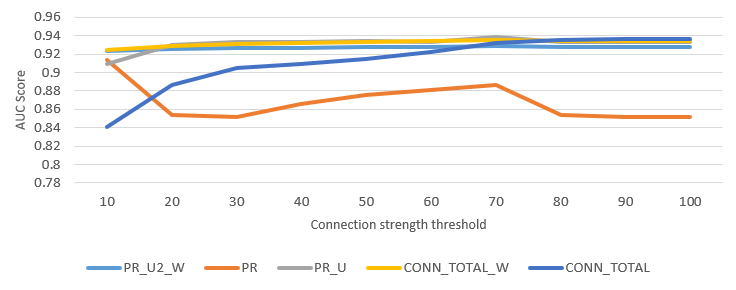
\includegraphics[width=\textwidth]{ant_SD_LD.PNG}
\caption{Variation of AUC score when varying connection strength threshold for Ant. Results for structural and logical dependencies combined. }
\label{fig:plot_sd_ld_ant}
\centering
\end{figure}


\begin{figure}
\centering
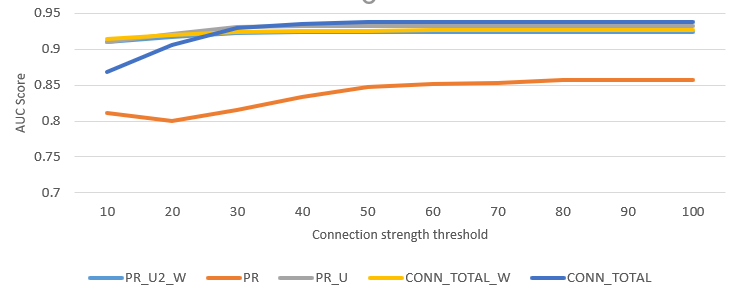
\includegraphics[width=\textwidth]{tomcat_SD_LD.PNG}
\caption{Variation of AUC score when varying connection strength threshold for Tomcat. Results for structural and logical dependencies combined. }
\label{fig:plot_sd_ld_tomcat}
\centering
\end{figure}


\begin{figure}
\centering
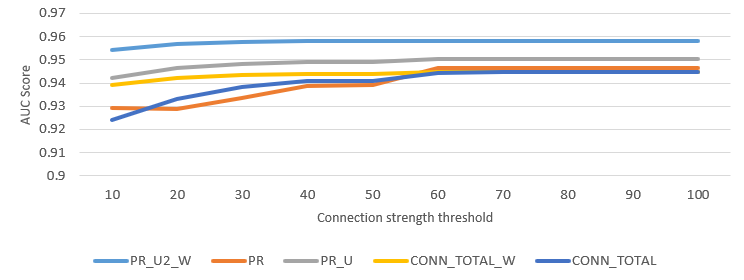
\includegraphics[width=\textwidth]{hibernate_SD_LD.PNG}
\caption{Variation of AUC score when varying connection strength threshold for Hibernate. Results for structural and logical dependencies combined. }
\label{fig:plot_sd_ld_hibernate}
\centering
\end{figure}



\begin{figure}
\centering
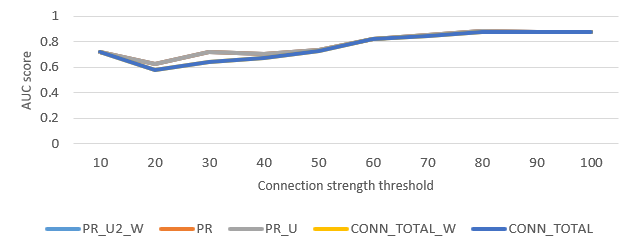
\includegraphics[width=\textwidth]{ant_LD.PNG}
\caption{Variation of AUC score when varying connection strength threshold for Ant. Results for logical dependencies only. }
\label{fig:plot_ld_ant}
\centering
\end{figure}


\begin{figure}
\centering
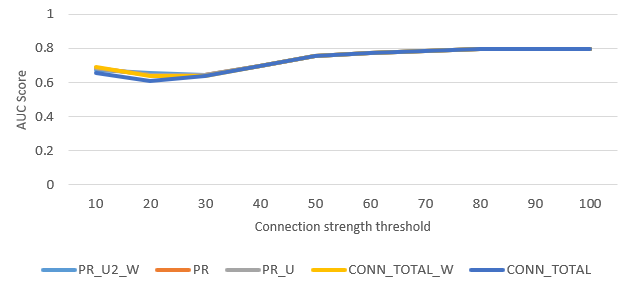
\includegraphics[width=\textwidth]{tomcat_LD.PNG}
\caption{Variation of AUC score when varying connection strength threshold for Tomcat. Results for logical dependencies only. }
\label{fig:plot_ld_tomcat}
\centering
\end{figure}


\begin{figure}
\centering
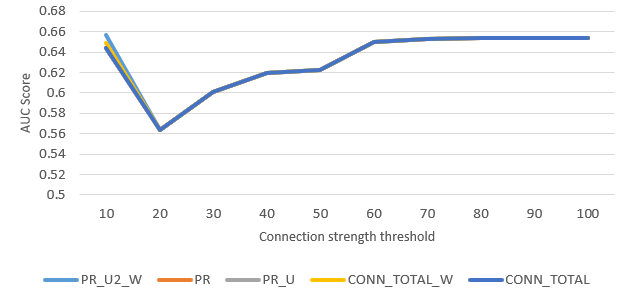
\includegraphics[width=\textwidth]{hibernate_LD.PNG}
\caption{Variation of AUC score when varying connection strength threshold for Hibernate. Results for logical dependencies only.}
\label{fig:plot_ld_hibernate}
\centering
\end{figure}


The details of the systems are presented in two tables.  In table \ref{tab:overlap} are the overlappings between structural and logical dependencies expressed in percentages. Each column represents the percentage of logical dependencies that are also structural, for each column the logical dependencies are obtained by applying a different connection strength filter. The connection strength filter begins at 10, meaning that in at least 10 \% of the total commits involving two entities, the entities update together. We increase the connection strength filter by 10 up until we reach 100, meaning that in all the commits that involve one entity, the other entity is present also.


In table \ref{tab:ratio_sd_ld} are the ratio numbers between structural dependencies and logical dependencies. We added this table in order to highlight how different the total number of both dependencies is.


\begin{table}[!h]
\renewcommand{\arraystretch}{1}
\caption{Percentage of logical dependencies that are also structural dependencies}
\label{tab:overlap}
\centering
\begin{tabular}{|c|cccccccccc|}
\hline
System &	$\geq10\%$	&	$\geq20\%$		&	$\geq30\%$		&	$\geq40\%$		&	$\geq50\%$		&	$\geq60\%$		&	$\geq70\%$		&	$\geq80\%$		&	$\geq90\%$		&	$\geq100\%$ \\
\hline
Ant	&	25.202	&	34.419	&	36.385	&	34.656	&	33.528	&	33.333	&	28.659	&	33.333	&	35.294	&	35.294	\\
Tomcat Catalina	&	4.059	&	22.089	&	25.000	&	25.758	&	25.926	&	37.525	&	47.368	&	55.285	&	75.000	&	76.923	\\
Hibernate	&	6.546	&	26.607	&	29.565	&	32.374	&	32.543	&	45.170	&	44.980	&	42.473	&	42.473	&	42.473	\\
\hline
\end{tabular}
\end{table}



\begin{table}[!h]
\renewcommand{\arraystretch}{1}
\caption{Ratio between structural and logical dependencies (SD/LD)}
\label{tab:ratio_sd_ld}
\centering
\begin{tabular}{|c|cccccccccc|}
\hline
System &	$\geq10\%$	&	$\geq20\%$		&	$\geq30\%$		&	$\geq40\%$		&	$\geq50\%$		&	$\geq60\%$		&	$\geq70\%$		&	$\geq80\%$		&	$\geq90\%$		&	$\geq100\%$ \\
\hline
Ant	&	1.315	&	3.284	&	4.972	&	5.603	&	6.175	&	10.697	&	12.915	&	27.154	&	41.529	&	41.529	\\
Tomcat Catalina	&	0.120	&	0.923	&	1.313	&	1.531	&	1.619	&	3.177	&	7.092	&	13.146	&	67.375	&	124.385	\\
Hibernate	&	1.037	&	6.391	&	10.037	&	14.947	&	18.940	&	54.248	&	83.442	&	111.704	&	111.704	&	111.704	\\

\hline
\end{tabular}
\end{table}

In figures \ref{fig:plot_sd_ld_ant}, \ref{fig:plot_sd_ld_tomcat} and \ref{fig:plot_sd_ld_hibernate} are the measurements obtained by using structural and logical dependencies combined. 
In all three figures, the measurements at the beginning are smaller than the rest. Once with the increasing of the threshold value also the measurements begin to increase. Meaning that better results for key class detection are found. 
The best measurements are when the threshold value is between 40 and 60, after that, the measurements tend to decrease a little bit and stay at that fixed value. 

A possible explanation of the results fluctuation and then capping is that if we are looking at table \ref{tab:ratio_sd_ld} we can see that at the beginning, the total number of logical dependencies used is close to the number of existing structural dependencies. The high volume of logical dependencies introduced might cause an erroneous detection of the key classes, in consequence, smaller measurements. 
When the threshold begins to be more restrictive and the total number of logical dependencies used begins to decrease, the key classes detection starts to improve. This improvement stops after the threshold value reaches 60\%. If we look again at table \ref{tab:ratio_sd_ld} we can see that after 60\% the number of structural dependencies outnumbers the number of logical dependencies up to 124 times in some cases. In addition, if we look at table \ref{tab:overlap} we can see that the remaining logical dependencies overlap a lot with the structural dependencies, so we are not introducing too much new information.

 So, the number of logical dependencies used is so small that it doesn't influence the key class identification. Since the structural dependencies used don't change, we obtain the same results for different threshold values. 



In figures \ref{fig:plot_ld_ant}, \ref{fig:plot_ld_tomcat} and \ref{fig:plot_ld_hibernate} are the measurements obtained by using only logical dependencies.
Initially, we expected to see a Gaussian curve, but instead, we see a bell curve.  We think that in the beginning, we use a high number of logical dependencies in key class detection, among those logical dependencies is an important number of key classes and also an important number of other classes. But the number of other classes does not influence the key classes detection. When we start to increase the value of the threshold and filter more the logical dependencies, we also filter some of the initial detected key classes and remain with a significant number of other classes. In this case, the other classes that remain influence the measurements, causing the worst-performing solutions. 
Some of the key classes are strongly connected in the versioning system, and even for higher threshold values don't get filtered out. Meanwhile, the rest of the classes that are not key classes get filtered out for higher threshold values which leads to better performing measurements when the threshold value are above 60\%. 

\section{Conclusions}
\label{sec:conclusion}


The logical dependencies are filtered co-changing pairs extracted from the versioning system history. The filters applied to the co-changing pairs are the following: the filter based on commit size and the filter based on connection strength.

In our experiments the filter based on commit size had a hard threshold of 10 files, meaning that we use co-changing pairs only from commits with at most 10 files changed. The filter based on connection strength had a variable threshold, starting with 10\% and ending with 100\%. We used a variable threshold for connection strength because we wanted to observe how this threshold will impact the key classes detection.

In section \ref{sec:current_measurements} we approached two scenarios to detect key classes by using logical dependencies. In the first scenario, we used logical dependencies together with structural dependencies and in the second, we used only logical dependencies to detect the key classes. We modified the tool used in the baseline approach to use also logical dependencies, and then we performed the key class identification using that tool. 
The quality of the results obtained was evaluated with the same tool, the metric used to evaluate the results is Area Under the Receiver Operating Characteristic Curve (ROC-AUC). We then compared the evaluation results with the results obtained by the baseline approach. 

Based on the results obtained, compared with the baseline results, we did saw a slight improvement in key class detection when both logical and structural dependencies were used together, the best results were obtained with a connection strength threshold of 40-70\%. When we used only logical dependencies to detect key classes, the results were less performing than using only structural or structural and logical dependencies combined.

As we mentioned in section \ref{sec:baseline_approach}, also other researchers tried to identify the key classes, and even though the approaches are not the same, most of them have used the ROC-AUC metric to evaluate the quality of the results. 
Osman et al. obtained in their research an average Area Under the Receiver Operating Characteristic Curve (ROC-AUC) score of 0.750 \cite{6676885}. Thung et al. obtained an average ROC-AUC score of 0.825 \cite{rocclasification}  and Sora et al. (the baseline approach) obtained an average ROC-AUC score of 0.894 \cite{Finding-key-classes}.

In the current research, we obtained an average ROC-AUC score of 0.926 when using logical and structural dependencies combined and a score of 0.747 when using only logical dependencies to detect key classes.

In conclusion, by using both dependencies combined, we can obtain a slightly better ROC-AUC score than the one obtained by the baseline approach. And, by using only logical dependencies we don't obtain a better score than the baseline approach but compared with the results obtained by other researchers \cite{6676885}, the score obtained is almost equal. The advantage of using only logical dependencies in key class detection is that it only uses data extracted from the versioning system and can be generalized to various programming languages.




\bibliographystyle{splncs03}
\bibliography{logicaldepd}


%%%%%%%%%%%%%%%%%%%%%%%%%%%%%%%%%%%%%%%%%
%% For the final version of the paper: %%
%%%%%%%%%%%%%%%%%%%%%%%%%%%%%%%%%%%%%%%%%

%% Author information
%\vspace{4ex}\noindent
%\textbf{Author One} is\dots
%
%\bigskip\noindent
%\textbf{Author Two} is\dots
%
%\bigskip\noindent
%\textbf{Author Three} is\dots

%% Reception and acceptance information
%\bigskip
%\paragraph{Received: Month DD, 20YY; Accepted: Month DD, 20YY.}

\end{document}
